\documentclass[12pt]{article}
\usepackage{ctex} % 支持中文
\usepackage{geometry}
\usepackage{amsmath}
\usepackage{graphicx}
\usepackage{booktabs}
\usepackage{hyperref}
\usepackage{float} % 用于控制表格位置
\usepackage{longtable}


\geometry{a4paper, margin=0.4in,bottom=0.5in}

\title{OCT-PIV流速测量实验}
\author{毛川伟}
\date{\today}

\begin{document}
\maketitle

\section{研究背景}

PIV,全称为微粒子图像测速。基本原理是通过一个相机连续拍摄在溶液当中的示踪粒子。通过对比连续拍摄到的图片,计算前一张图片到后一张图片的相关性。找到相关位移。然后通过标定,得到实际和像素之间的关系
通过这个关系来计算流速。下面是PIV的基本原理图

\begin{figure}[h]
    \centering
    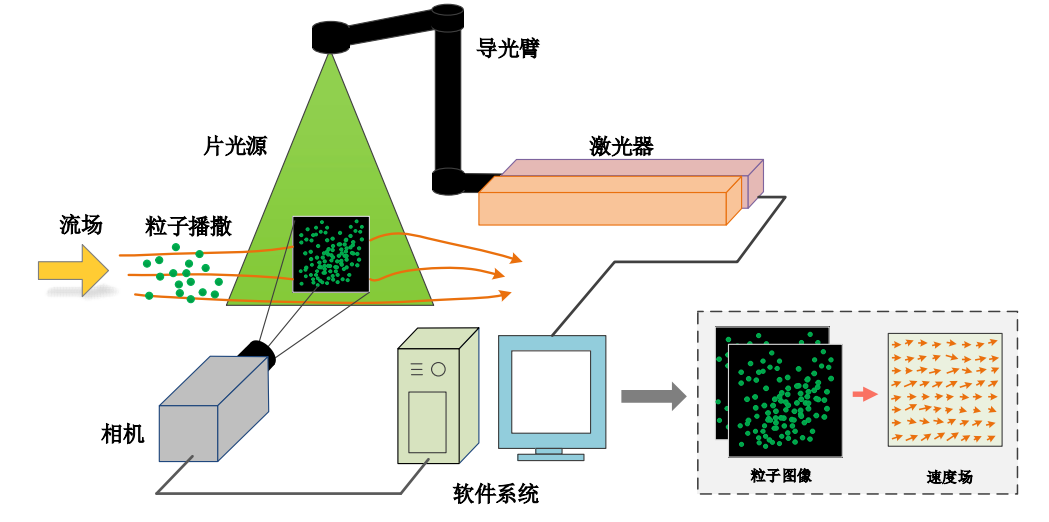
\includegraphics[width=0.8\textwidth]{Images/PIV_principles.png}
    \caption{粒子图像测速技术工作原理示意图}
    
    
\end{figure}

PIV的计算公式如下,


    \begin{equation}
        R(x,y)=\sum_{i=-L}^L\sum_{j=-L}^LI(i,j)I'(i+x,j+y)
    \end{equation}

    其中$I(.)$和$I'(.)$分别为前后帧图像提取的窗口像素灰度值。第一幅图中的查询窗口称为模板,利用模板在第二幅图像的搜索范围中进行不断的遍历和匹配,就
    可以得到相关平面

    \begin{figure}
        \centering
        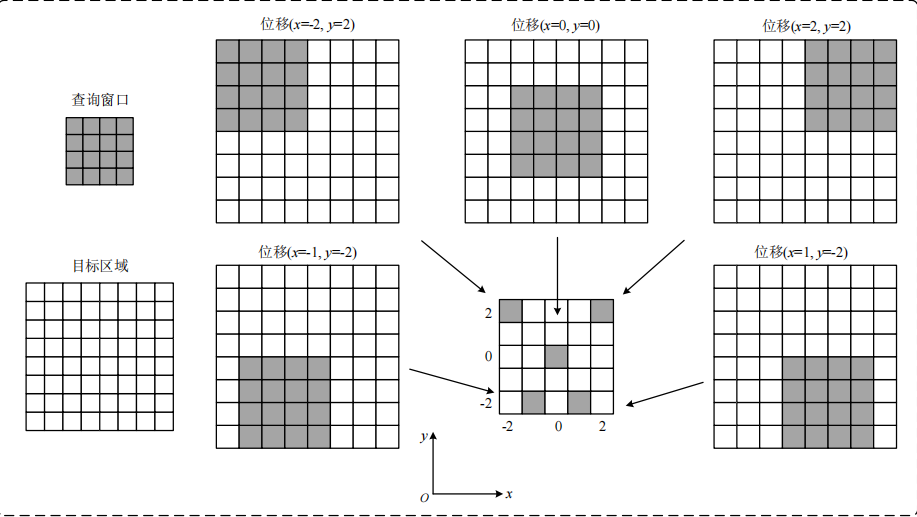
\includegraphics[width=0.8\textwidth]{Images/互相关算法示意图.png}
        \caption{互相关 PIV 算法的计算原理示意图}
        
        
    \end{figure}

    \begin{figure}
        \centering
        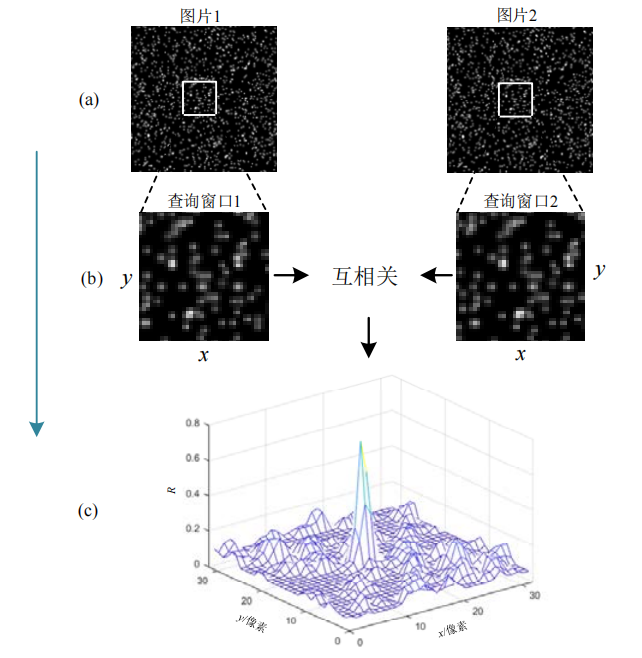
\includegraphics[width=0.8\textwidth]{Images/互相关示意图.png}
        \caption{互相关算法计算的互相关平面}
        
    \end{figure}
    

\section{实验目的}
\begin{itemize}
    \item 测试PIV测速的可行性
    \item 验证PIV

\end{itemize}

\section{实验内容}
\begin{itemize}

    \item 制作玻璃管流道
    \item 使用聚苯乙烯微球作为示踪粒子,配置聚苯乙烯微球溶液
    \item 设置不同的灌流流速,使用OCT设备采集数据
    \item 使用PIVlab工具包计算流场和速度
    \item 将得到的流场和预先设置值进行对比,计算均值和方差,分析该方法得到的结果
\end{itemize}



\section{实验材料和设备}
\subsection{材料清单}



{
    \footnotesize
    \begin{longtable}{@{} p{5cm} p{10cm} @{}}
        \toprule
        \textbf{材料} & \textbf{备注} \\ 
        \midrule
        
        
        聚苯乙烯微球        & 用来作为示踪粒子\\
        玻璃管两根          & 作为微流道,一根备用\\
        橡胶管两条              & 用来连接注射器,微流道,和灌流器 \\
        灌流器              & 用来设置灌流流速 \\
        琼脂粉              & 和水混合加热到沸腾,等到30-40°冷却就会凝固\\
        一个离心管的瓶盖    & 用于放置玻璃管\\
        微波炉              & 用于加热琼脂 \\
        天平                 & 在使用之前需要在放上称量纸的情况下调零 \\ 
        移液枪               & 在配置材料实验室里 \\ 
        离心管(2个)        & 用于配置聚苯乙烯微球溶液 \\ 
        称量纸               & 方便倒出材料   \\
        5ml 注射器(4个)    & 存放聚苯乙烯微球溶液 \\ 
        灌流器               & 位于三楼实验室抽屉 \\ 
        空心橡胶管(2条)    & 长度不能够太短 \\ 
        3D 打印注射器喷头    & 红色,套在注射器上用于连接橡胶管 \\ 
        纯净纸巾             & 用来擦拭漏出的溶液 \\ 
        
        一把剪刀            & 用来剪断橡胶管 \\
        
        \bottomrule
        \caption{实验材料列表} \\
    \end{longtable}
}




\section{实验流程}

\subsection{准备材料}
\begin{itemize}
  
    \item 提前带上U盘或者移动硬盘
    \item 提前预约实验室
    \item 提前打开实验室的新风系统(中间控制面板),以及空调系统(在门左右边)
    \item 带上聚苯乙烯微球材料
\end{itemize}
\subsection{配材料}
\begin{enumerate}
    \item 琼脂溶液的配置
    \begin{itemize}
        \item 百分之5的琼脂溶液,取10g琼脂粉,灌水到200ml
        \item 加入一点牛奶(不能够加太多,会降低透光度)
        \item 使用微波炉加热琼脂到沸腾
       

    \end{itemize}
    \item 制作带缺口瓶盖
    \begin{itemize}
        \item 取下一个离心管的瓶盖
        \item 使用小刀刻出缺口
    \end{itemize}

    \item 配置聚苯乙烯微球溶液
    \begin{itemize}
        \item 配置百分之10质量的微球溶液
        \item 取5g聚苯乙烯微球,使用移液枪添加45ml取离子水
        \item 需要搅拌均匀
    \end{itemize}
\end{enumerate}

\subsection{开始实验}
\begin{enumerate}
    \item 材料的装配
    \begin{itemize}
   
    \item 使用5ml的注射器吸入聚苯乙烯微球溶液
    \item 将材料都放到同一个实验架子上,并做好区分,这样不用到处找材料
    
    \end{itemize}

    \item 制作直流通道
    \begin{itemize}
        \item 从微波炉当中取出溶液,倒入瓶盖当中并等待凝固(注意琼脂不要太厚,应该稍微覆盖即可,否则会降低透光率)
        \item 连接金属管和橡胶管
    \end{itemize}

    \item 搭建灌流平台
    \begin{itemize}
        
        \item 将直流通道和灌流设备连接起来
        \item 往流道里面注入溶液
        \item 设置不同的灌流流速,使用如下公式来计算对应流速的灌流量,其中L表示灌流量,单位是ul/min,r表示半径,单位是mm,
        v表示流速,单位是mm/s。其中,玻璃管的内半径是0.45mm。根据这个公式设置对应的灌流量,每组流速重复测量4次。届时可以计算均值和方差
        \begin{equation}
            L=60 \pi r^2 v
        \end{equation}

       \footnotesize
       \begin{longtable}{@{} p{5cm} p{5cm} p{5cm} @{}}
           \toprule
           \textbf{OCT数据序号} & \textbf{流速 mm/s} & \textbf{灌流量 ul/min} \\ 
           \midrule
           1 & 0 & 0 \\
           2 & 0 & 0 \\
           3 & 0 & 0 \\
           4 & 0 & 0 \\
           5 & 1 & 38.17 \\
           6 & 1 & 38.17 \\
           7 & 1 & 38.17 \\
           8 & 1 & 38.17 \\
           9 & 2 & 76.34 \\
           10 & 2 & 76.34 \\
           11 & 2 & 76.34 \\
           12 & 2 & 76.34 \\
           13 & 3 & 114.51 \\
           14 & 3 & 114.51 \\
           15 & 3 & 114.51 \\
           16 & 3 & 114.51 \\
           17 & 4 & 152.68 \\
           18 & 4 & 152.68 \\
           19 & 5 & 152.68 \\
           20 & 5 & 152.68 \\
           \bottomrule
           \caption{流速设置表格} \\
       \end{longtable}

    
    \end{itemize}

    \item 开始采集数据
    \begin{itemize}
        \item 等到流速稳定之后开始采集数据
        \item 找到像,我们应该找到正像,通过显微镜镜头找到正像(从摄像头看,显微镜达到对扫描物体的聚焦比较清楚),然后将物体移动到强度最高的位置(注意,会呈现两个像,一个正像一个反像,这是由于光程差存在正反
        (注意:对于具有强反射率的玻璃表面,我们的成像可能会存在两条横杠,这个玻璃的反光,可能会影响最终的成像)
        \item 调整像素个数,让成像更加清晰,或者通过固定像素实际大小和视场来自动得到像素值
        \item 开始采集数据2D界面数据(之所以采集2D,是为了测试该方法的可行性。
        \item 通过实验室的电脑将图片导出来。共同保存到Images文件夹当中
        \item 每个灌流量,需要重复采集4次(为了后面建立方差和均值模型)
        \item 实验采集数据完毕
    \end{itemize}

    \item 实验结束准备
    \begin{itemize}
        \item 将不要的东西都扔到垃圾桶当中
        \item 将灌流器收起来放到抽屉当中
        \item 关闭实验室的新风系统,关闭实验室的空调(新风系统显示连锁关闭,空调在左右门)
        \item 将OCT设备关机(注意,先关闭计算机,才关闭OCT设备)
        \item  将垃圾到到6楼的垃圾筒当中去
    \end{itemize}

    \section{数据处理}


    \subsection{算法简介}
    \begin{itemize}
    \item 集成相关PIV算法。为了防止有的地方没有粒子或者粒子较少导致的速度测量不准确的问题。为了能够准确测量位移。需要综合多次的测量结果。
    \begin{figure}
        \centering
        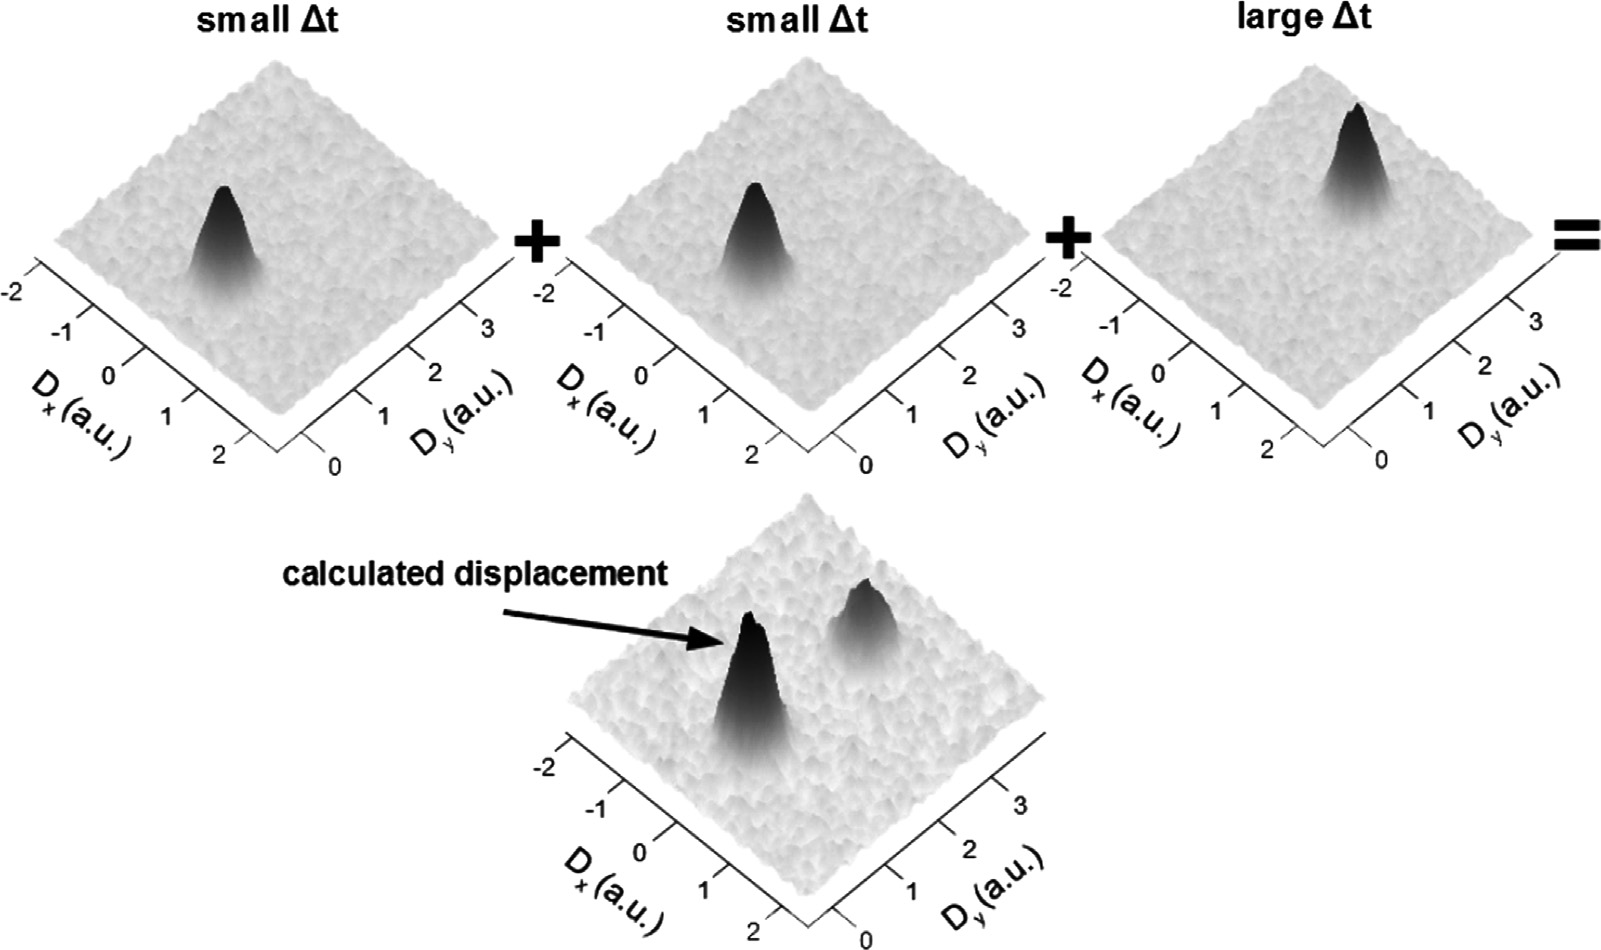
\includegraphics[width=0.8\textwidth]{Images/累加PIV原理展示.png}
        \caption{累加PIV原理展示}
    \end{figure}
    \item 多窗口PIV。为了能够更加精细地反映流速。我们使用了多窗口。逐步加大流场的精细度,如下图所示
    
    \begin{figure}
    \centering
    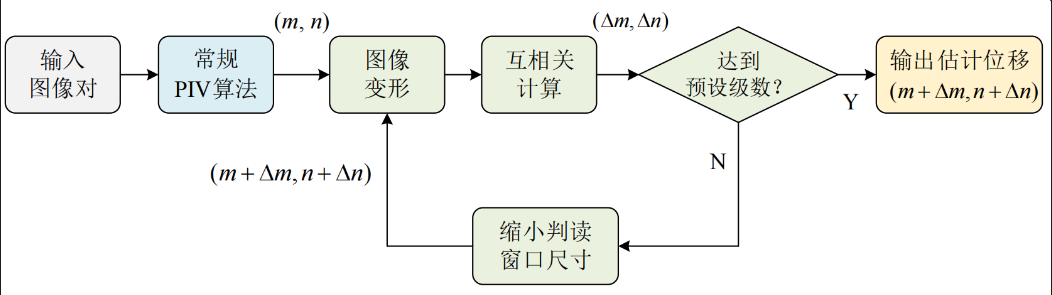
\includegraphics[width=0.8\textwidth]{Images/多窗口示意图.png}
    \caption{多窗口计算流程图}
    \end{figure}

    \end{itemize}
    \subsection{Matlab—PIVlab计算流速}
    \begin{enumerate}
        \item 将从公司得到的数据放到自己电脑上
        \item 将图片导入到PIVLab当中
        \item 选择PIV算法。这次我们选择集合相关PIV算法,通过集成100张图片来进行计算
        \item 对图像进行校准。将像素尺寸映射到现实当中(可以通过OCT测量流道的尺寸,然后,标定对应的尺寸,从而得到流速)
        \item 进行后处理:去除不想要的流速
        \item 绘图,绘制出相应的流场图,流场图包括流速幅值等等。
        
        \begin{figure}
            \centering
            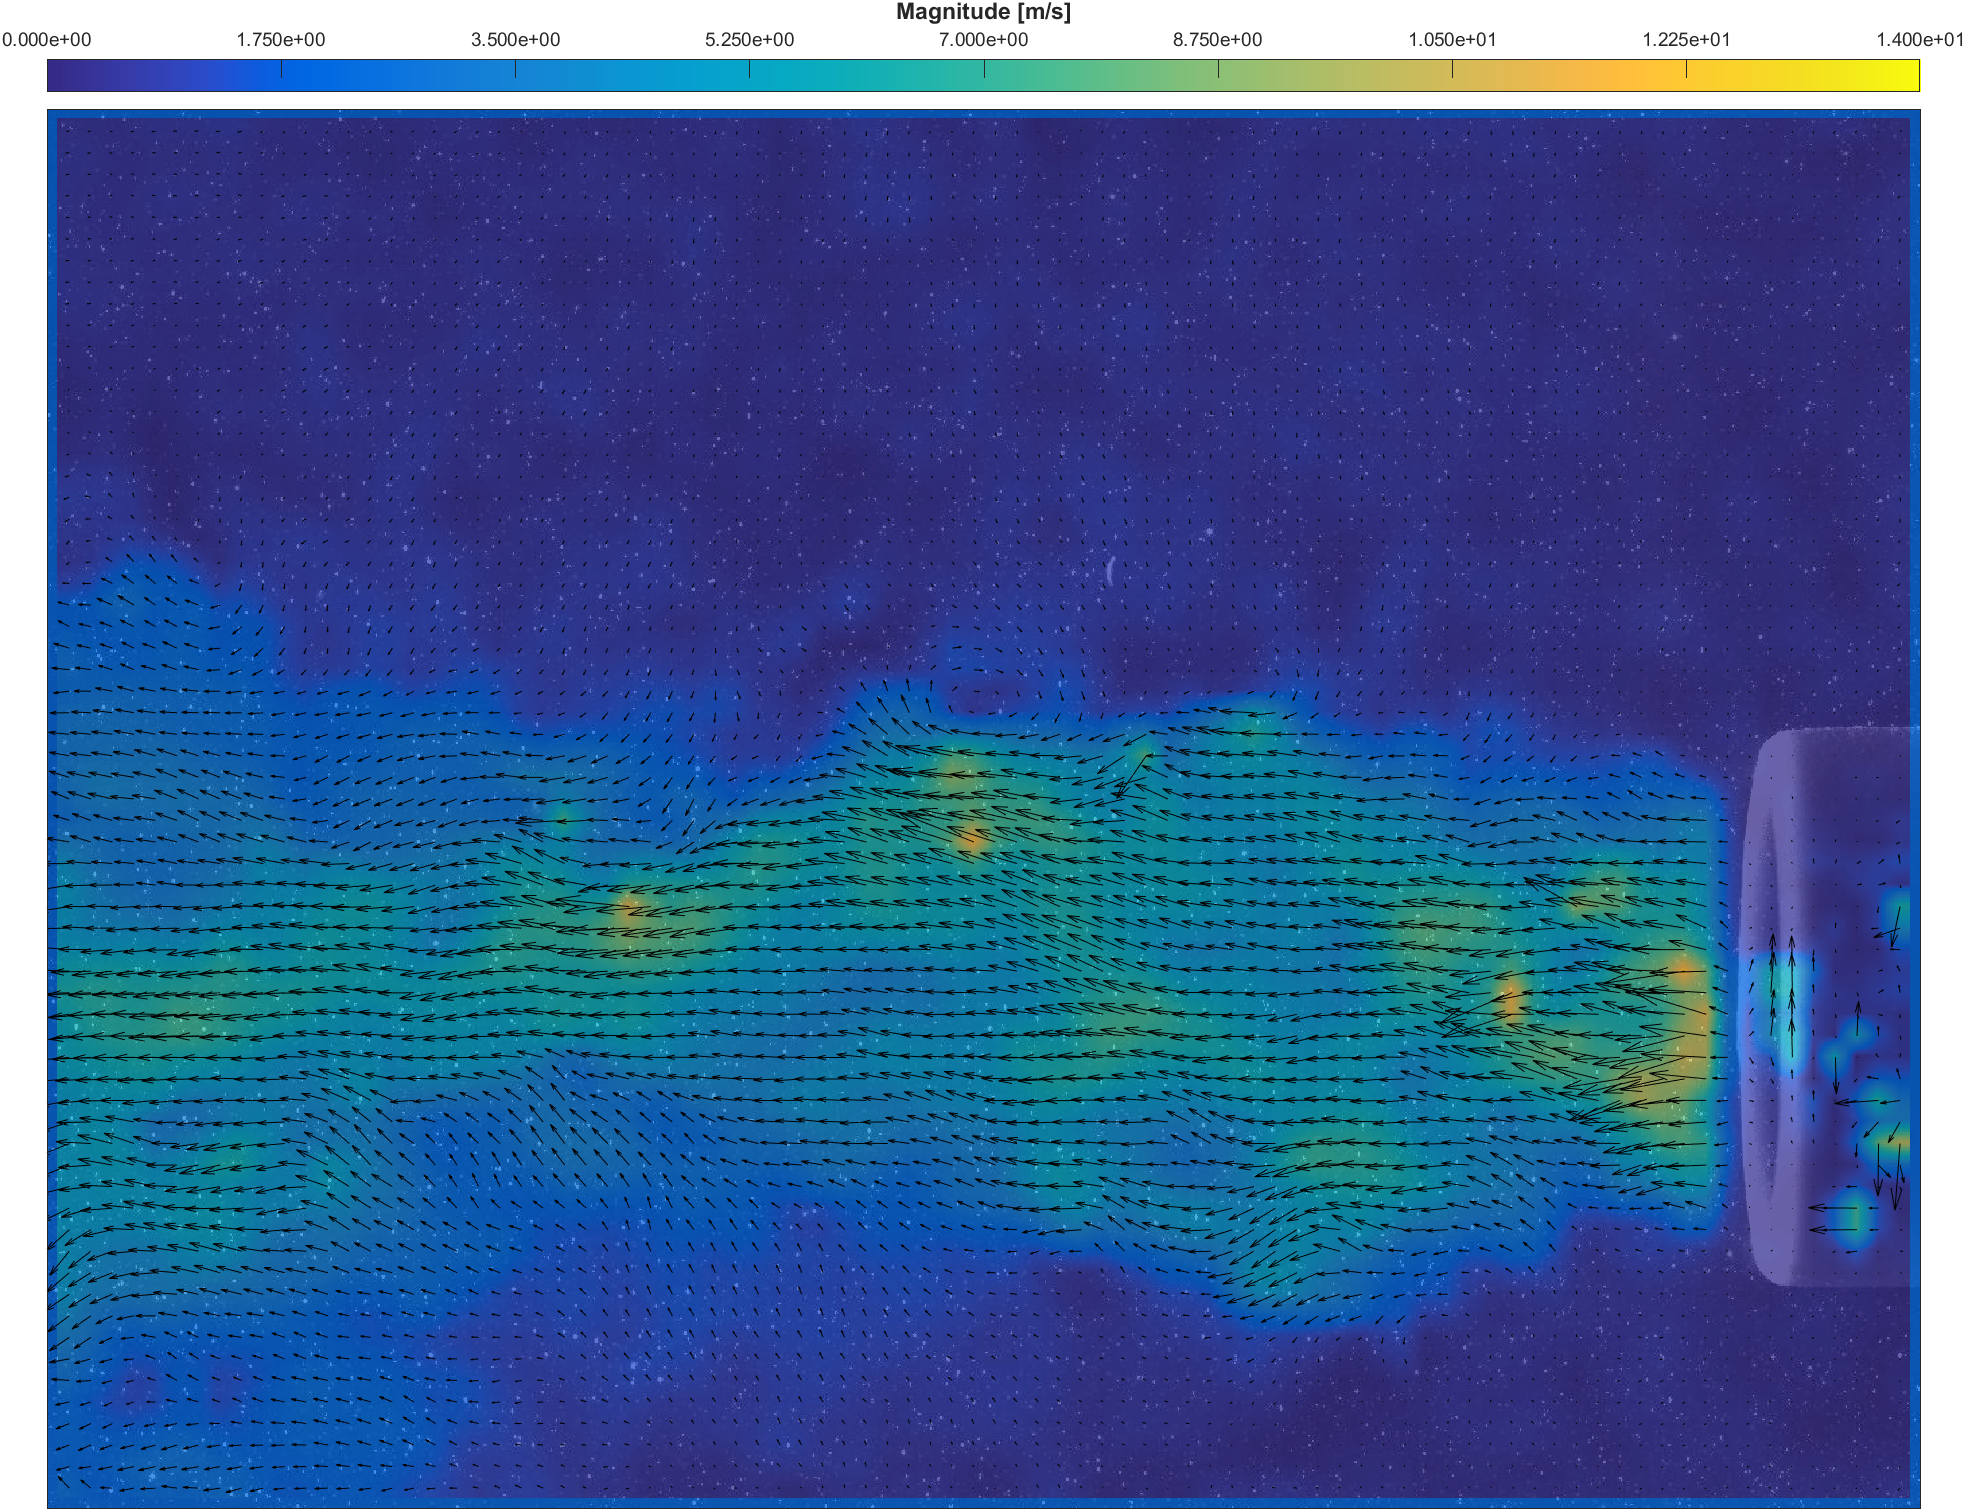
\includegraphics[width=0.8\textwidth]{Images/经过Matlab处理后的图片.png}
            \caption{计算出来的流场示意图}
        \end{figure}
        \item 提取出来相应的信息用来分析流场,包括散点图等等东西
        \item 通过PIV提取出来感兴趣区域的流速均值,在数据预处理部分,或者后面的画图进行展示
        \item 根据多组流速计算流速的方差。
        \item 我们最终会导出该过程用到的各种数据,到我们的工作表当中,根据工作表,我们也能够进行分析
    \end{enumerate}
    


\section{可能的意外与应对措施}
\begin{itemize}

    \item 配材料室没开门(等待 可能有人在休息)
    \item 中间遇到的会议(看情况,如果会议紧急的话先去开会议,否则可以请假)
\end{itemize}

\section{参考文献}

\begin{itemize}
    \item 基于 CCd-OCTA 的三维流场成像技术及其对3D打印类血管网的研究 
    \item Vista
    \item Complex differential variance algorithm for optical coherence tomography angiography
    \item Improved motion contrast and processing efficiency in OCT angiography using complex-correlation algorithm
\end{itemize}

\end{document}